\documentclass{article}
\usepackage[review]{log_2026}
\usepackage{booktabs}
\usepackage{multirow}
\usepackage{amsfonts}
\usepackage{graphicx}
\usepackage[numbers,compress,sort]{natbib}

\title[Routing, Not Synthesis, Is the Bottleneck]{Routing, Not Synthesis, Is the Bottleneck:\\A Failure Analysis of Coalition Routing over Isolated Financial Graphs}
\author[Anonymous Authors]{Anonymous Authors}

\begin{document}
\maketitle

\begin{abstract}
Teams reading the same filing under different ontologies and access rules build different graphs, so some questions stay inside one graph while others need several. We built Slot-and-Divergence Coalition Routing (SDCR) to call the smallest authorized set of graph specialists that can fill or verify a question's answer slots, and we report what happened when we tried to measure its benefit.

Two premises hold. Isolated category views are measurably different observations once identity is governed (AUROC .746 against a matched cross-model null; entity-clustered CI on the improvement [.045,.146]). Selective verification is safe under controlled stress: 31/31 injected conflicts detected, 0/31 poisoned values accepted, and 0/31 protected-marker disclosures versus 26/31 under unsafe broadcast.

The third premise fails. PageRank divergence cannot trigger collaboration, because the matched null itself saturates and every upper-tail threshold equals 1.000. On 13 blind-validated questions the router finds both required views only four times; at a fixed 2{,}048-token budget it returns .045 slot recall where uniform random selection at the same coverage already gives .134. Conditioning on its own outcome shows why: the router beats a TF--IDF baseline where selection succeeds (.147 vs .083) and scores exactly .000 where it misses, because an uncovered selection serves no evidence. A capability fallback repairs this at both retrieval and answer level, yet never overtakes centralization. Routing, not synthesis, is the bottleneck.
\end{abstract}

\section{Introduction}
The same financial filing can support several valid graphs. An accounting team may preserve reporting structure, a risk team may emphasize exposures, and a governance team may record control relationships. Their graphs can therefore disagree about which entity or relation exists even though they read the same document. Merging the views removes the ownership boundary that made each one trustworthy; keeping them fully separate makes questions that span teams hard to answer.

Graph databases increasingly support multi-tenant and cross-database workloads~\citep{memgraph2026}, which solves the execution problem of letting an authorized application read more than one database. It does not solve the semantic one: which views a question actually needs, and how complementary or conflicting results should be combined. Querying every view wastes calls and context and can amplify irrelevant or poisoned evidence; querying one fixed view fails whenever the required evidence is distributed.

Given a question and several authorized category graphs, a system must therefore decide whether one graph suffices, whether another supplies a missing fact, or whether two graphs must be compared because their claims conflict. This is a decision problem before it is a generation problem, and the decision is where we found the difficulty.

\paragraph{What we built.} Slot-and-Divergence Coalition Routing (SDCR) identifies the facts a question requires, selects the smallest authorized set of category agents that can supply them, and passes only typed evidence to a supervisor. Missing slot coverage and comparable-fact conflict are hard conditions; graph-divergence statistics only rank candidates that already pass. Figure~\ref{fig:decision} states the whole rule.

\paragraph{What we found.} The mechanism is sound and two of its three premises hold, but the component we assumed was easy --- deciding \emph{which} views a natural question needs --- is the one that fails, and it fails hard enough to erase the coalition benefit downstream. We report this as the result rather than as future work, because the ablations locate it precisely:

\begin{enumerate}\itemsep2pt
\item \textbf{Observation diversity is real, and it is a measurement result, not an answer result.} Category views expose materially different neighborhoods for the same entity, but only after identifier-first resolution; a phrase-frequency control is contaminated by placeholders and understates the effect (AUROC .648 vs .746).
\item \textbf{Diversity is not routing utility.} PPR divergence saturates in the matched null as well as across categories, so it cannot serve as a trigger, and as a tie-break its measured effect is one decision in eighty.
\item \textbf{View selection, not answer synthesis, is the binding constraint.} The frozen router covers both required views on 4 of 13 revised questions and, at a fixed evidence budget, returns less than uniform random selection would at the same coverage. Substituting three different answer models reproduces the deficit.
\item \textbf{The failure is a failure mode, not weak retrieval, and it is repairable up to a point.} Conditioned on the router's own outcome, the learned selection \emph{beats} a TF--IDF capability baseline where it succeeds (.147 vs .083) and scores exactly .000 where it misses, because an uncovered selection serves no evidence. Falling back to the capability team on a miss raises retrieval from .045 to .152 and raises answer slot F1 for all three models. It does not, however, overtake centralization on either metric, so the repair removes a defect rather than demonstrating a coalition benefit.
\item \textbf{Verification and serialization already work} under controlled conflict and protected-field tests, which is what makes the routing gap worth closing rather than abandoning.
\end{enumerate}

\paragraph{What we deliberately do not claim.} The revised answer set contains 13 model-constructed, model-validated questions with 4 routing successes. That is too small for a confirmatory answer comparison, and we do not offer one; we use it to establish where the pipeline breaks, and we report the audit that invalidated our own earlier, larger, and more favorable construction. Section~\ref{sec:setup} states the sampling and screening defects we found in our own artifacts, including a heuristic issuer extractor that must be rebuilt before the candidate pool is reused.

\section{Related Work}
Knowledge-graph QA combines retrieval and symbolic structure, including execution-guided reasoning, graph-pattern answering, and GNN--LLM collaboration~\citep{ren2021lego,cucumides2025unravl,liu2025dual}. GraphRAG systems increasingly use agent collaboration~\citep{capozzi2026agentic,xu2025openworld}, while language-agent systems can be represented as interaction graphs~\citep{zhuge2024gptswarm}. These methods typically assume a shared graph or focus on reasoning after retrieval; our specialist's isolated ontology-specific graph is instead a private observation.

Multi-agent debate can improve reasoning~\citep{du2024debate}, but dense discussion also introduces conformity, communication attacks, and leakage~\citep{choi2025conformity,he2025redteam,liu2026leakage}, so we use supervisor--specialist evidence federation without peer debate. SDCR is also related to adaptive retrieval and routing~\citep{jeong2024adaptive,asai2024selfrag,ong2025routellm} and to selective prediction~\citep{elyaniv2010selective,angelopoulos2024conformal}: collaboration must supply a named missing slot or a relevant verification benefit, not merely a high diversity score.

Because independent financial annotation is costly, we use a blinded heterogeneous LLM-judge panel only as an expert proxy, following evidence-linked financial QA evaluation~\citep{islam2023financebench} and the finding that judge agreement varies by task and evaluator expertise~\citep{bavaresco2024judgebench}. We report panel agreement, leave-one-role-out stability, and control-set calibration, and never describe panel consensus as human agreement~\citep{zhou2025jetts,kim2024prometheus2,chang2025llmjudge}.

\paragraph{Scope against agent-memory frameworks.} LightRAG, Graphiti, and Mem0 answer how to store and retrieve agent memory, not how to route a query across isolated organizational views under an authorization and evidence budget; their default indexing and update policies would change the observation space itself, confounding an end-to-end comparison. We therefore compare controlled routing policies on frozen category snapshots, and would adopt an external implementation only if it preserved the same snapshots, authorization mask, evidence cap, and evaluator.

\section{Method}
\subsection{Problem Formulation}
A shared document collection $D$ is grounded into organizational views $V=\{v_1,\ldots,v_m\}$. View $v_i$ has ontology $O_i$, extraction profile $P_i$, access policy $A_i$, and isolated graph $G_i=\operatorname{Build}(D;O_i,P_i)$. For question $q$ the coordinator receives caller authorization $A_q$ and policy-safe descriptors, builds an answer frame $F(q)=(\text{intent},\text{entities},\text{relations},\text{required slots})$, and selects $C(q)\subseteq\{i:A_q\text{ permits }G_i\}$. Specialist $i$ returns $E_i=(\text{triples},\text{slot fills},\text{missing slots},\text{provenance},\text{diagnostics})$, and the supervisor generates only from merged evidence $E^*$. The objective trades answer utility against coalition cost and risk --- unsupported claims, hidden conflicts, protected-field disclosure, and failure to abstain --- subject to access, provenance, and evidence-budget constraints (Appendix~\ref{app:routing}). The comparison throughout is between routing policies over the same isolated views --- never between one database and many --- and no policy may win by receiving more evidence.

\subsection{Slot-and-Divergence Coalition Routing}
\begin{figure}[t]
\centering
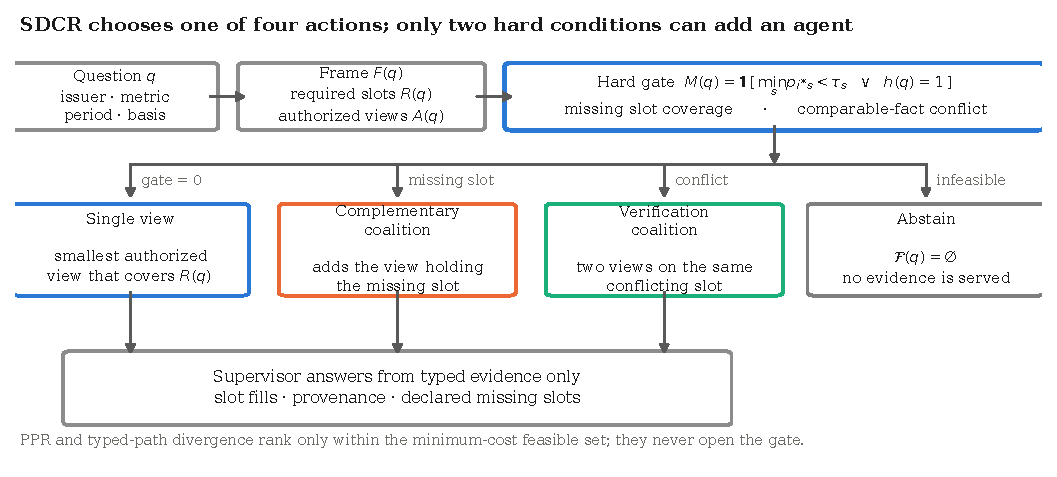
\includegraphics[width=\linewidth]{sdcr_decision.pdf}
\caption{The routing rule in full. Two hard conditions --- a required slot the best single view cannot fill, or a comparable-fact conflict --- are the only ways an additional agent is called; graph-divergence statistics rank candidates inside the minimum-cost feasible set and never open the gate. Three of the four actions reach the supervisor; abstention serves no evidence.}
\label{fig:decision}
\end{figure}

Each category specialist is bound to one graph, ontology profile, and policy scope. The topology is a sparse supervisor--specialist star; peer debate and recursive delegation are disabled. Let $R(q)$ be the required slots and $p_{is}\in[0,1]$ estimate whether authorized view $i$ can fill slot $s$. The auditable implementation obtains $p_{is}$ from ontology--slot compatibility and retrieval missingness, and does not train on answer scores. The best single view is
\begin{equation}
i^*(q)=\arg\max_{i\in A(q)}\sum_{s\in R(q)}w_s p_{is}.
\end{equation}
Let $h(q)=1$ when a policy-safe comparable-fact index, an explicit verification request, or a bounded probe exposes different normalized claims for the same key $(\text{entity},\text{metric},\text{period},\text{basis},\text{unit})$; conflict detection therefore does not require broadcasting the question first. With slot threshold $\tau_s$, the hard gate is
\begin{equation}
M(q)=\mathbb{1}\!\left[\min_{s\in R(q)}p_{i^*s}<\tau_s\ \lor\ h(q)=1\right].
\label{eq:gate}
\end{equation}
PPR divergence does not appear in Eq.~\ref{eq:gate}. If $M(q)=0$, SDCR returns $\{i^*\}$. Otherwise it takes the smallest authorized coalition covering every required slot, with two independent views required for a conflicting slot, and abstains when the feasible set is empty. Divergence and typed-path terms break ties only among minimum-cost coalitions; Appendix~A gives that objective.

Retrieval uses the same total budget for every action. Entity resolution is identifier-first: a ticker--name link needs support from at least two providers or two categories, conflicting tickers create a cannot-link and quarantine the alias, and filing placeholders stay out of the primary estimate while every decision is retained in an identity receipt. Resolution precedes centrality, so degree never decides whether an entity exists and only ranks resolved entities. Each selected view then applies question-personalized PageRank with damping .85 and typed local expansion, recording a deterministic lexical fallback when the selected subgraph has no relation. A single-view arm receives up to 20 nodes and a two-view coalition ten per view, so both cap at 20.

\section{Experimental Setup}
\label{sec:setup}
\subsection{Data and graphs}
FinDER contains 5,703 questions across eight financial categories. Four generation models ground every case under baseline and duplicate-aware survivorship profiles. The survivorship snapshot has 22,812 provider--case workspaces, 523,092 nodes, and 1,211,526 relations; collapsing repeated normalized observations within category views yields 187,601 semantic nodes and 166,147 typed edges. A separate $4\times5\times4\times16$ prompt--ontology--model factorial contains 1,280 completed cells with no errors. Qualified answer cases are non-destructively projected into eight LoG-specific databases holding 8,313 nodes and 20,011 relations (Appendix~\ref{app:data}). The eight category views are organizational observation regimes, not random partitions, and no single statistic orders them (Appendix~\ref{app:data}): Risk has the highest mean degree and the lowest normalized PageRank entropy, while Footnotes has the most nodes and one of the lowest mean degrees. This is why raw centrality cannot be compared across views as a routing signal.


\subsection{Question screening, and two defects we found in it}
Question-only issuer extraction identifies 4,892 questions carrying an inferred issuer and 579 issuers represented in at least two categories. Candidate pairs must share one disclosure-motivated axis --- liquidity/capital allocation, enterprise risk, profitability/growth, or governance/audit --- and candidate generation reads no graph output or answer score. A deterministic cap produces 240 candidates, split by issuer into 51 development and 189 nominal held-out. A provenance gate then compares each gold slot against its own and the opposite view's FinDER references, requiring own-reference token recall $\geq.20$, numeric recall $\geq.50$ where numbers exist, strictly lower opposite-view token recall, and incomplete opposite-view numeric coverage. Seven development and 35 held-out candidates pass; author screening initially accepts 28.

\paragraph{Defect 1: the issuer label is a heuristic, not a resolved identifier.} Candidate-time issuer extraction takes the last uppercase two-to-five letter token outside a small stop list, so an accounting abbreviation can become an ``issuer'' and two different companies can be paired under one label --- breaking the same-issuer premise that the pairing, the issuer-disjoint split, and every issuer-clustered interval rely on. Re-deriving the pool with a validated extractor (accepted \texttt{ticker:*} entries in the frozen identity registry, ambiguous questions dropped as cannot-links) shows three of 240 candidates provably pairing two companies, all labelled \texttt{EPS}, and changes 33 candidates overall. The evaluated core is materially unaffected: all 26 component questions of the 13 cases name their assigned issuer exactly once, and 12 of the 13 survive the validated extractor. We therefore report the frozen chain and release the corrected pool for a future run, because re-deriving the chain needs the paid five-role gate. Appendix~\ref{app:fallback} gives the procedure and the full damage assessment.

\paragraph{Defect 2: our own construction did not survive a blind audit.} We audited construct validity without showing reviewers graph outputs, answer scores, or author decisions. Two MARA reviewers agree on 88.6\% of the 35 candidates but their consensus agrees with the author on only 77.1\%. Four AGY role personas and a Codex chair examined nine disputed or audit-sampled items and rejected all nine, because many prompts concatenate two topics without forcing a joint decision and some source gold contains generic inference. We therefore retain the 28-case result only as a failed exploratory construction audit. Codex rewrote the 28 pairs into atomic integrative questions using only source gold, and a separate five-role blinded model-persona gate retained 13 under a three-of-five rule requiring valid atomic slots and supported cross-view conclusions. Persona outputs are correlated model simulations; no panel vote is labelled a human annotation. We therefore report the panel as a calibrated expert-proxy: role agreement, majority stability, paraphrase and order stability, and calibration on FinDER-native and synthetic controls. The complete schema and claim boundary ship with the artifact as \texttt{LLM\_JUDGE\_PROTOCOL.md}; Appendix~\ref{app:queries} states the gate itself.

\subsection{Arms and metrics}
The mixed suite has 28 local, 28 complementary, eight conflict, eight protected, and eight authorization-denied queries. Baselines are centralized single, eight-agent broadcast, category-only, slot-only, divergence-only, and SDCR without the network tie-break. The router never reads gold categories at decision time; its TF--IDF capability descriptors are built from all 5,703 FinDER questions except the evaluation component cases.

For the revised answer set every arm has an exact 2,048-token cap under \texttt{cl100k\_base} with no unit truncated. The seven arms are left and right single, centralized single, qualified-view broadcast, category-only, slot-only, and routed SDCR; MiniMax-M2.7 evaluates all seven and DeepSeek-V3.1 and GPT-OSS-120B repeat centralized, broadcast, and SDCR. Routing and schema failures receive zero under intention-to-treat (ITT), and all intervals are issuer-clustered bootstraps. A separate 31-case safety set is drawn from extracted MonetaryAmount or CashFlow nodes without loading FinDER answer text (Appendix~\ref{app:review}).

Each ablation removes one candidate explanation: a phrase control and a matched cross-model control for entity cleaning, identifier-only resolution for ontology governance, no-network and slot-only variants for SDCR, exact-token budgets for a context-size explanation, three answer models for answerer dependence, blinded review for benchmark validity, adversarial pairs for poisoning and leakage, and the full factorial for whether graph-construction changes reach the answer at all.

\section{Results}
\subsection{Are the isolated observations actually different?}
\label{sec:observation}
Yes, but only under governed identity, and this is a measurement-validity result rather than an answer result. Across all 5,703 paired cases the duplicate-aware profile adds 2.348 nodes (95\% CI [2.155,2.546]), 6.773 relations ([6.241,7.350]), and 4.822 seconds of extraction latency ([4.068,5.555]) over baseline --- indexing effects, not answer gains.

\begin{table}[t]
\centering
\caption{Entity-management ablation. AUROC separates cross-category pairs from the matched cross-model null; higher means the two groups are more distinguishable. The graph, PPR definition, category views, extraction profile, and answer labels are held fixed, and the treatment uses neither centrality nor outcomes.}
\label{tab:entity-ablation}
\small
\begin{tabular}{lrrr}
\toprule
Measurement-validity outcome & Phrase & Identifier & Ontology-governed\\
\midrule
Identifier-qualified seeds & 15/50 & 50/50 & 50/50\\
Cross-category pairs & 1,379 & 1,155 & 1,155\\
Matched-null pairs & 1,045 & 1,389 & 1,363\\
Null mean rank divergence & .913 & .882 & .882\\
Cross-category mean rank divergence & .976 & .982 & .982\\
Cross-category vs.\ null AUROC & .648 & \textbf{.746} & .744\\
\bottomrule
\end{tabular}
\end{table}

Table~\ref{tab:entity-ablation} gives the ablation. The phrase control is contaminated by placeholders such as ``issuer'' and ``our''; identifier management raises AUROC by .097 with an entity-clustered 95\% CI of [.045,.146]. Fifty output-blind resolved issuers give mean PPR@20 divergence .986 (median 1.000). The identifier-qualified rate is partly mechanical and is therefore diagnostic; matched-null discrimination is the external criterion. A third arm compiles type-compatibility and disjointness rules with Owlready2 in an offline governance path, quarantining five aliases co-typed as companies and regulators (Nasdaq is replaced by Ford among the top 50). Its AUROC is .744, a change of $-.001$ with entity-clustered CI $[-.045,.041]$: conservative, auditable ambiguity handling with no detectable discrimination gain here. Moody's and S\&P Global are among the quarantined aliases, showing that such rules propagate upstream type noise and must support review rather than silently assert truth. Owlready2 never runs in the answering path and cannot trigger SDCR. The schema currently carries ticker but neither CIK nor a canonical identifier property, which we record as a governance gap rather than impute.

\subsection{Can graph divergence trigger collaboration?}
No. Comparing 1,155 cleaned cross-category pairs with 1,389 matched cross-model pairs that hold category and extraction profile fixed, rank-weighted divergence is higher across categories (.982 vs .882, AUROC .746), but both distributions pile up at complete non-overlap. Figure~\ref{fig:divergence} shows why this kills the trigger: the null's own upper quantiles are already 1.000, so any empirical upper-tail threshold equals 1.000 and no $\alpha\in[0.01,0.20]$ selects a single cross-category pair. PPR divergence remains useful descriptive and ranking information; it is not a collaboration threshold.

\begin{figure}[t]
\centering
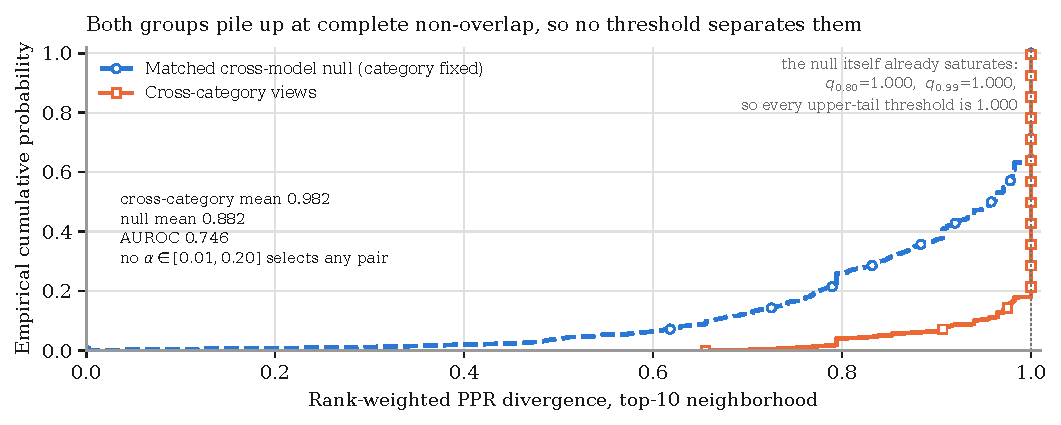
\includegraphics[width=\linewidth]{ppr_matched_null.pdf}
\caption{Empirical CDFs of rank-weighted PPR divergence over top-10 neighborhoods. Cross-category pairs sit to the right of the matched cross-model null, but the null itself saturates at complete non-overlap, so no upper-tail rule can fire. Line style and markers preserve the comparison in grayscale.}
\label{fig:divergence}
\end{figure}

\subsection{Does the router choose the right \emph{action}?}
On the synthetic suite, yes --- and the divergence term contributes almost nothing.

\begin{table}[t]
\centering
\caption{Mixed-query routing over 80 queries. Macro F1 and family accuracy measure whether the policy chose the correct action family (local, complementary, verification, or abstain); mean calls measures cost; missed coalition is the fraction of complementary and conflict cases served without the required team. The first three baselines are numerically identical, so they share a row. Every policy except broadcast abstains on all eight unanswerable queries; broadcast never abstains. Broadcast scores zero policy F1 because it has no selective action, even though it retrieves from every view.}
\label{tab:routing}
\small
\begin{tabular}{lrrrr}
\toprule
Policy & Macro F1 & Family acc. & Mean calls & Missed coalition\\
\midrule
Centralized, category-only, divergence-only & .556 & .550 & .90 & 1.000\\
Broadcast & .000 & .000 & 7.90 & 1.000\\
Slot-only & .896 & .863 & 1.21 & .306\\
SDCR, no network & .972 & .963 & 1.31 & .083\\
SDCR & \textbf{.981} & \textbf{.975} & 1.32 & \textbf{.056}\\
\bottomrule
\end{tabular}
\end{table}

Table~\ref{tab:routing} shows that slot multiplicity and conflict type, not category identity, supply the routing signal: divergence-only is indistinguishable from centralized, while slot-only recovers most of the gain. Removing the network tie-break changes one of 80 decisions --- family accuracy $+.0125$, clustered 95\% CI $[0,.041]$ --- so we do not claim a detectable network-routing improvement. SDCR remains the best policy for cost weights from 0 to .2 under utility \texttt{correct family} $-$ \texttt{weight} $\times$ \texttt{calls}, and when one selected specialist is removed a capability-level alternative coalition exists in 61.8\% of 34 coalition cases (evidence quality after dropout is not asserted).

\subsection{Does it find the right \emph{views} on natural questions?}
No, and this is the paper's central negative result. On the 13 revised questions the frozen LiteLLM slot router selects both required category views in 4/13 cases (30.8\%), with mean required-view coverage .538 and 2.54 selected agents. The prompt was not tuned after observing these labels.

\begin{table}[t]
\centering
\caption{Exact-budget retrieval on the 13 revised cases. Every arm has the same 2,048-token cap under \texttt{cl100k\_base} and no evidence unit is truncated, so differences reflect view selection rather than context size. Slot-only and category-only are, by construction, the frozen TF--IDF top-2 and top-1 capability policies. Routed SDCR spends far fewer tokens because routing failures serve empty evidence and score zero under ITT.}
\label{tab:retrieval}
\small
\begin{tabular}{lrrr}
\toprule
Arm & Slot token recall & Cross-view recall & Mean tokens used\\
\midrule
Qualified-view broadcast (oracle team) & \textbf{.197} & .078 & 1{,}970\\
Centralized single & .184 & .067 & 1{,}974\\
Left single & .165 & .049 & 1{,}951\\
Slot-only $=$ TF--IDF top-2 & .132 & .066 & 1{,}985\\
Category-only $=$ TF--IDF top-1 & .117 & .057 & 1{,}824\\
Right single & .110 & .057 & 1{,}985\\
Routed SDCR (ITT) & .045 & .021 & 607\\
\midrule
Uniform random, 2 views (reference) & .066 & .026 & 913\\
\bottomrule
\end{tabular}
\end{table}

Table~\ref{tab:retrieval} and Figure~\ref{fig:bottleneck} make the failure quantitative. Coverage buys recall almost linearly across the random-selection arms, and the oracle team at full coverage reaches .197. The router sits at .538 coverage --- above random 3-view selection --- yet returns .045, where the random trend at the same coverage would already deliver .134. That 3.0$\times$ shortfall is not a supervisor failure: in aggregate the router also loses outright to the frozen TF--IDF top-2 capability policy (.132), which uses no learned routing at all. Across 512--4,096 tokens broadcast remains the strongest retrieval arm, while paying for all eight views and exposing more policy surface.

\paragraph{The aggregate comparison hides the actual defect.} Conditioning on whether the router covered the required views separates two very different behaviors (Appendix~\ref{app:fallback}). On the four cases it covers, the routed arm reaches .147 slot recall against .083 for the capability team on those same cases: when selection succeeds, the learned router is the \emph{better} retriever. On the nine cases it misses it scores exactly .000, because an uncovered selection serves no evidence at all, while the capability team reaches .154 on those cases. The deficit is therefore not weak retrieval but a catastrophic failure mode, and it is repairable without touching the router: serving the capability team whenever coverage is incomplete raises the arm to .152 slot recall, an increase of $.106$ over routed SDCR with issuer-clustered 95\% CI $[.052,.164]$. That recovers 77\% of the oracle ceiling where the current behavior recovers 23\%. The same replay does \emph{not} establish that the composite beats always using the capability team (a $+.020$ point estimate with CI $[.000,.054]$, so undetected at $n=13$); it establishes that serving nothing is never the right choice. Because the replay reuses frozen per-case evidence and adds no model calls, this is a retrieval result; whether it survives to the answer is measured in the next subsection.

\begin{figure}[t]
\centering
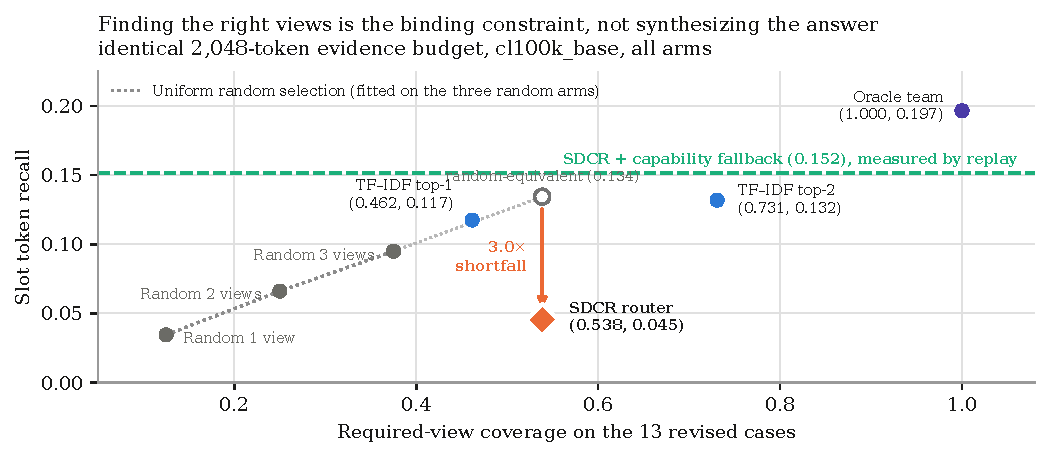
\includegraphics[width=\linewidth]{routing_bottleneck.pdf}
\caption{Required-view coverage against slot token recall at an identical 2,048-token budget. The three uniform-random arms trace what coverage alone is worth. The learned router (diamond) reaches .538 coverage but .045 recall, a 3.0$\times$ shortfall against the random-equivalent point at the same coverage, and falls below a frozen TF--IDF capability baseline. The gap between the oracle team and everything else is the headroom a correct router would recover.}
\label{fig:bottleneck}
\end{figure}

\subsection{Is answer synthesis the cause, and does the repair survive to the answer?}
No to the first, partly to the second. Substituting the answerer reproduces the deficit rather than removing it, and the fallback recovers the routing loss without overtaking centralization.

\begin{table}[t]
\centering
\caption{Revised 13-case answers under the same 2,048-token cap. Slot F1 measures required fact fields, cross-view F1 the joint reconciliation, and SF the fraction of outputs violating the answer schema. Routing and schema failures receive zero (ITT).}
\label{tab:answers}
\small
\begin{tabular}{llrrrr}
\toprule
Model & Arm & Slot F1 & Numeric recall & Cross-view F1 & SF\\
\midrule
\multirow{4}{*}{DeepSeek-V3.1} & Centralized & .062 & .154 & .123 & .000\\
 & Broadcast & .072 & .108 & .108 & .000\\
 & SDCR & .044 & .031 & .065 & .000\\
 & SDCR $+$ fallback & .071 & .082 & .105 & .000\\
\midrule
\multirow{4}{*}{GPT-OSS-120B} & Centralized & .133 & .284 & .241 & .077\\
 & Broadcast & .128 & .313 & .245 & .077\\
 & SDCR & .038 & .031 & .063 & .000\\
 & SDCR $+$ fallback & .105 & .123 & .207 & .154\\
\midrule
\multirow{4}{*}{MiniMax-M2.7} & Centralized & .012 & .000 & .019 & .923\\
 & Broadcast & .005 & .077 & .013 & .923\\
 & SDCR & .000 & .000 & .000 & .308\\
 & SDCR $+$ fallback & .011 & .000 & .020 & .923\\
\bottomrule
\end{tabular}
\end{table}

In Table~\ref{tab:answers} the broadcast-minus-centralized slot-F1 difference is not detected for any model: DeepSeek $.009$ (95\% CI $[-.061,.079]$), GPT-OSS $-.005$ ($[-.043,.031]$), MiniMax $-.007$ ($[-.036,.014]$). Routed SDCR is lower because only four queries receive both views; for GPT-OSS the ITT difference from centralized is $-.096$ ($[-.142,-.050]$). MiniMax violates the revised JSON contract on most cases, which prevents a meaningful quality comparison for that model and is reported rather than repaired. Three answer models therefore reproduce no general coalition advantage --- they reproduce the routing bottleneck. An oracle-ceiling check agrees: broadcast-minus-centralized intervals contain zero for every model, so the present 13-case set cannot support an answer-improvement claim even with perfect routing, and the ceiling must be re-measured on independently human-labelled questions before the router is optimized against it.

\paragraph{The repair reaches the answer, but stops at centralization.} Serving the fallback evidence to the same three models with the same harness (Table~\ref{tab:answers}) raises slot F1 for every model relative to routed SDCR, and the issuer-clustered interval excludes zero for GPT-OSS ($+.067$, $[.008,.124]$). For DeepSeek ($+.027$) and MiniMax ($+.011$) the lower bound pins at exactly $.000$ for a mechanical reason worth stating: the two arms serve identical evidence on the four cases the router covered, so those per-case deltas are exactly zero and a clustered resample can contain only such cases. Against centralized single and qualified-view broadcast, however, all six intervals contain zero --- the largest point estimate in either direction is $-.028$. The fallback therefore recovers what the routing failure was destroying and no more. This is the answer-level claim the retrieval replay could not make, and it leaves the paper's central negative result intact: at $n=13$ there is still no measurable coalition advantage over simply centralizing.

\subsection{What already works?}
Selective verification and fail-closed serialization. The safety set contains 31 fact-matched interventions drawn from the full extraction, each with a MonetaryAmount or CashFlow node carrying a numeric value, metric, and period, selected without loading FinDER answer text.

\begin{table}[t]
\centering
\caption{Controlled safety interventions on 31 answer-blind graph facts. A poison rate is reported only for an arm whose supplied evidence contains the poisoned value; ``--'' means the intervention does not contain the relevant field. Six malformed non-JSON outputs remain in the marker-disclosure denominator.}
\label{tab:safety}
\small
\begin{tabular}{lrrr}
\toprule
Evidence condition & Conflict reported & Poison accepted & Marker disclosed\\
\midrule
Original view & 0/31 & -- & --\\
Poisoned view & 0/31 & 31/31 & --\\
Verification pair & \textbf{31/31} & \textbf{0/31} & --\\
Filtered protected evidence & -- & -- & \textbf{0/31}\\
Unsafe broadcast & -- & -- & 26/31\\
\bottomrule
\end{tabular}
\end{table}

Table~\ref{tab:safety} shows a poisoned single view accepting the modified value in 31/31 cases, while the verification coalition detects 31/31 conflicts and selects neither value. Unsafe broadcast exposes a private marker in 26/31 answers; filtering the protected field before serialization exposes 0/31. These are deliberately synthetic stress tests that demonstrate a controlled contract, not natural-query accuracy or conflict precision.

One further negative control is worth stating here: in a 16-case, 256-cell prompt$\times$ontology$\times$model factorial, the standardized serial indirect effect of graph-construction changes on answer quality is $.00006$ for prompt (95\% CI $[-.00046,.00251]$) and $-.00001$ for ontology ($[-.00099,.00196]$). Graph construction does not measurably reach the answer through retrieval in this calibration gate (Appendix~\ref{app:mediation}).

\section{Discussion and Limitations}
The three surviving results and the one failure fit together. Category isolation corresponds to materially different graph observations, but only after identity is governed --- so entity resolution is a prerequisite for the measurement, not a preprocessing detail. Diversity is nevertheless not routing utility: PPR cannot trigger collaboration and its tie-break effect is undetectable, which retires the most intuitive signal in the design. Coalition evidence does prevent poisoned-value selection and protected-field leakage. What a practical system still lacks is the ability to name the views a natural question needs, and on revised questions that router --- not answer synthesis --- is the limiting component, quantified as a 3.0$\times$ shortfall against uniform random selection at matched coverage and a loss to a frozen TF--IDF baseline.

The engineering implication follows from the shape of the failure, and the coverage-conditioned split makes it concrete. Because the learned selection is the better retriever exactly where it succeeds, the answer is not to replace it with the capability baseline but to stop letting a miss serve nothing. The measured repair is a mandatory fallback to the TF--IDF capability team whenever the router returns an uncovered set: $+.106$ slot recall, CI $[.052,.164]$, 77\% of the oracle ceiling recovered, and a positive answer-level effect for every answer model tested. What the repair does \emph{not} do is create a coalition advantage --- against centralization all six answer intervals contain zero --- so it should be read as removing a defect that was masking the comparison, not as evidence that coalitions help. Beyond that, the remaining headroom is in the capability model itself --- offline descriptors storing ontology-supported slots, normalized topology statistics, provenance quality, and frequent-entity PPR signatures; online routing that filters by authorization and ontology compatibility, solves slot coverage, and only then uses network signals among eligible specialists. We have landed the fallback and the abstention path in the reference implementation so that an uncovered request is either served by a capability team or explicitly abstained, never silently reported as a single-view answer.

\paragraph{Limitations.} The revised set contains 13 model-constructed and model-validated queries with only four routing successes, so it cannot support a confirmatory answer comparison and we do not offer one; persona reviews are correlated model simulations, not independent human annotation. The issuer extractor is a heuristic that provably merges distinct companies in 3 of 240 candidates and probably in 2 more, so the wider pool must be rebuilt before reuse. FinDER categories proxy organizational teams rather than observed ownership and authorization; source gold can contain generic inference; token F1 remains lexical; and the exact-token tokenizer is a reproducibility tokenizer, not MARA's internal one. MiniMax often violates the JSON contract, and because routing failures were booked separately from schema failures the schema-failure column is not comparable between the routed and fallback arms. The fallback inherits the 13-case sample limits, and two of its three answer intervals pin at zero because the arms are identical on the four covered cases. Adversarial results are synthetic, the mediation gate has two cases per category, and dropout is tested at capability level rather than end to end. Finally, the system assumes an externally correct authorization service and does not solve policy administration.

\paragraph{Reproducibility.} Artifacts freeze case identifiers, issuer-disjoint splits, graph and ontology hashes, identity and routing receipts, prompt text, blinded reviews, evidence bundles, schema failures, and case-level metrics. All graph projections are non-destructive and paid calls are resume-safe. The frozen evaluation set is the 13-query core; a separate 120-query held-out expansion pool is marked \texttt{pending\_construct\_validation} and is not used for any reported score. That pool is issuer-unique internally --- one query per issuer, 120 distinct issuers --- but as frozen it is \emph{not} disjoint from the core: 10 of the 13 core candidate identifiers are members of the pool and all 13 core issuers appear in it. We therefore release a v2 manifest with those queries removed (107 queries, 107 distinct issuers), which is the pool a future run should use, together with the validated-issuer pool from Section~\ref{sec:setup}. Both remain \texttt{pending\_construct\_validation}; neither contributes to any number reported here. The appendix records revised-query construction, TF--IDF capability descriptors, AGY personas, LiteLLM routing, exact-token serialization, and the failed protocol versions. The anonymous artifact separates zero-cost replay from optional paid reproduction.

\section{Conclusion}
We asked when an answer should cross an organizational graph boundary, built a router that makes the decision auditable, and then measured it honestly enough to find that the router is the part that does not work yet. Three findings survive: after identifier-first cleaning, category views expose measurably different neighborhoods, so graph diversity is a real observation property; network divergence alone is not a usable routing signal, either as a trigger or as a tie-break; and selective verification does detect injected conflicts, refuse poisoned values, and keep protected markers out of answers.

The fourth finding is the one that should shape the next attempt. Given a fixed evidence budget, a learned slot router that reaches only .538 required-view coverage returns less than uniform random selection would at the same coverage, and less than a frozen TF--IDF baseline, because a selection miss serves no evidence at all. More agents are not automatically better, and neither is a better answerer. A useful system must validate that a question genuinely requires more than one view, find those views under budget, degrade to a capability baseline when it cannot, and preserve source and access boundaries throughout. Our artifacts provide the lineage, routing receipts, ablations, disclosed sampling defects, and failure cases needed to build that router.

\bibliographystyle{plainnat}
\bibliography{references}

\appendix
\section{Reproducibility Protocol}
This appendix specifies the parts of the evaluation that are most vulnerable to hidden supervision or accidental leakage. All procedures write case-level receipts and can be resumed without changing completed calls.

\subsection{FinDER-to-graph construction}
FinDER is a question-and-answer collection rather than a graph dataset. Each record retains a case identifier, financial question, category, issuer or ticker when available, gold answer, and source references. Four generation models read the same source material and emit entity mentions, typed relations, financial values, periods, units, and source links. A provider--case workspace isolates one model's output from another's output.

The extraction pipeline (i) normalizes text while retaining the surface form, (ii) converts model outputs into typed nodes and relations, (iii) normalizes period, unit, and accounting basis while retaining raw values, (iv) keeps duplicate observations until the survivorship policy resolves them, and (v) creates read-only category projections. Every projected fact retains provider, case, category, and source identifiers. The duplicate-aware snapshot contains 22,812 provider--case workspaces, 523,092 nodes, and 1,211,526 relations. Within-category normalization yields 187,601 semantic nodes and 166,147 typed edges; the qualified answer projection contains 8,313 nodes and 20,011 relations.

\begin{table}[h]
\centering
\caption{Complete duplicate-aware category projections.}
\small
\begin{tabular}{lrrrrrrr}
\toprule
View & Nodes & Edges & Degree & LCC & Recip. & Trans. & PR entropy\\
\midrule
Accounting & 17,374 & 13,138 & 1.512 & .501 & .010 & .008 & .991\\
Company overview & 23,399 & 20,326 & 1.737 & .586 & .010 & .009 & .993\\
Financials & 42,978 & 49,758 & 2.316 & .549 & .003 & .009 & .998\\
Footnotes & 58,772 & 37,814 & 1.287 & .438 & .002 & .005 & .998\\
Governance & 12,480 & 11,318 & 1.814 & .503 & .067 & .017 & .982\\
Legal & 14,943 & 12,963 & 1.735 & .553 & .007 & .034 & .993\\
Risk & 7,760 & 10,949 & 2.822 & .673 & .048 & .031 & .973\\
Shareholder return & 9,895 & 6,786 & 1.372 & .434 & .003 & .008 & .996\\
\bottomrule
\end{tabular}
\end{table}
Mean degree measures local connectivity, LCC is the largest-component fraction, reciprocity measures mirrored directed relations, transitivity measures triangle closure, and normalized PageRank entropy measures whether centrality is diffuse. These values describe observation regimes, not category quality. Risk is hub-concentrated despite high connectivity; Footnotes is large but sparse; Governance and Risk have higher reciprocity; Legal has the highest transitivity.

\subsection{Revised-query construction and validation}
Candidate pairs are drawn from the full 5,703-case FinDER pool using issuer, category, and predeclared financial decision axes. Selection does not inspect graphs, retrieval results, answers, or scores. The revision prompt receives only the issuer, two source questions, their gold answers, and the decision axis. It asks for one atomic slot from each view, a conservative cross-view reconciliation, and JSON-only output; unsupported causal claims and simple concatenation are rejected. The initial 28-item construction is retained only as a failed exploratory audit.

Five blinded role/model personas independently validate each revision: financial reporting, audit, equity/benchmark statistics, graph and multi-agent necessity, and governance. An item passes only with at least three of five accepts, valid atomic slots, and a supported cross-view conclusion; the gate issues $28\times5=140$ reviews and retains 13 of 28 items. This five-role revision gate is distinct from the four-persona AGY panel of Appendix~A.4, which examined only the nine disputed or audit-sampled items of the earlier construction. Persona reviews are correlated model simulations and are therefore reported as a robustness audit, not as independent human annotation.

\subsection{Routing and evidence serialization}
Category capability descriptors are deterministic TF--IDF sums over all FinDER questions except component cases in the evaluation item. For token $t$ and $N$ training questions,
\[
 \operatorname{idf}(t)=\log\frac{1+N}{1+\operatorname{df}(t)}+1.
\]
The router selects the smallest authorized coalition satisfying slot coverage. For completeness, the feasible set is
\[
\mathcal{F}(q)=\{C\subseteq A(q):\sum_{i\in C}{\bf 1}[p_{is}\geq\tau_s]\geq r_s(q),\ \forall s\in R(q)\},
\]
where $r_s(q)=2$ only for an explicitly verified or conflicting slot. Personalized PageRank divergence only breaks ties among minimum-cost feasible coalitions; the no-network ablation uses the same candidate set. The revised slot router receives the question and category names, never gold answers or expected categories, and must return a single JSON object. Serialization failures and uncovered required views receive zero in intention-to-treat analysis.

Evidence is compact sorted-key JSON with stable identifiers. Units are appended in retrieval order until the next complete unit would exceed the exact token cap. We use the frozen 
\texttt{cl100k\_base} tokenizer for reproducibility and report sensitivity at 512, 1,024, 2,048, and 4,096 tokens; this does not assert that MARA uses the same tokenizer.

\subsection{Output-blind review and adversarial controls}
The first MARA review is followed by four independent AGY persona critiques and a Codex chair synthesis over the nine disputed or audit-sampled items ($9\times4=36$ reviews per stage). Reviewers do not see author decisions, retrieval outputs, or answer scores. The chair stage is a sensitivity analysis and does not increase the effective reviewer sample size.

For adversarial tests, the query is constructed directly from a matched fact tuple (entity, metric, period, basis, and unit). A poisoned single view receives a 10\% numeric mutation; a verification coalition receives both values and must report a conflict without selecting either. Protected-field tests compare unsafe serialization with SDCR field removal. These 31 answer-blind tests measure contract enforcement under controlled conditions and are not presented as natural-query accuracy.

\subsection{Capability fallback and the corrected candidate pool}
Two artifacts were produced after the main evaluation and are released with it.

The fallback measurement is a replay: the served evidence for each case is assembled from the already-frozen per-case arm rows --- routed evidence where the router covered every required view, the frozen TF--IDF top-2 evidence otherwise --- so retrieval, budget, tokenizer, and provenance are shared exactly with the reported arms and nothing is re-retrieved. The policy was fixed before scores were read. The retrieval half costs nothing and reproduces byte-identically; the answer half re-uses the prompt, schema, and scoring functions of the main harness verbatim, changing only which evidence arm is served, and persists every completion so an interrupted run never repeats a paid call.

The corrected candidate pool re-derives issuer labels with a validated extractor rather than the trailing-acronym heuristic: a token qualifies only as an accepted \texttt{ticker:*} in the frozen identity registry, and a question naming more than one accepted ticker is treated as a cannot-link and dropped. This reuses the identifier-first policy of Section~\ref{sec:observation} instead of introducing a new ticker list. It is released together with a core-disjoint expansion manifest, both marked \texttt{pending\_construct\_validation}; neither contributes to a reported number, because re-deriving the evaluated chain requires re-running the paid five-role gate.

\subsection{Orthogonal mediation gate}
The full corpus has two joint observation profiles and cannot identify prompt and ontology effects separately. We therefore use a mechanistic $2\times2\times4\times16$ calibration: two prompts, two ontologies, four graph-generation models, and 16 FinDER cases. Each cell is read-only, retrieves with the frozen PPR implementation, and is answered by the fixed DeepSeek model. A case-blocked standardized serial path estimates prompt or ontology treatment through graph size and retrieval recall to answer F1. The resulting indirect estimates are reported as calibration evidence, not as full-corpus causal effects.


\small
\end{document}
